\documentclass[11pt]{article}

\usepackage{amsmath}
\usepackage{amsfonts}
\usepackage[margin=1in]{geometry}
\usepackage{enumitem}
\usepackage{graphicx}
\usepackage[colorlinks]{hyperref}
\usepackage{longtable}

\usepackage{helvet}
\renewcommand{\familydefault}{\sfdefault}

\setlength{\parindent}{0in}

\def\tightlist{}
\def\toprule{}
\def\bottomrule{}

\begin{document}

{\LARGE Homework 8 (Due November
11th)}\label{homework-8-due-november-11th}

{\Large 1. Bound charges and the
D-field}\label{bound-charges-and-the-d-field}

Consider a long teflon rod, (a dielectric cylinder), radius \(a\).
Imagine that we could somehow set up a permanent polarization
\(\mathbf{P}(s,\phi,z) = k\mathbf{s} ( = ks\hat{s})\), where \(s\) is
the usual cylindrical radial vector from the \(z\)-axis, and \(k\) is a
constant). Neglect end effects, the cylinder is long.

\begin{enumerate}
\def\labelenumi{\arabic{enumi}.}
\tightlist
\item
  Calculate the bound charges \(\sigma_{bound}\) (on the outer surface)
  and \(\rho_{bound}\) (in the interior of the rod). What are the units
  of your constant \(k\)? Show that the units work out in all formulas
  you have used involving \(k\).
\item
  Next, use these bound charges (along with Gauss' law, this problem has
  very high symmetry!) to find the electric field, \(\mathbf{E}\) inside
  and outside the cylinder. (Your answer should include both the
  direction and magnitude.)
\item
  Finally, determine the electric displacement field (\(\mathbf{D}\))
  inside and outside the cylinder using the fundamental definition
  (\(\mathbf{D} = \varepsilon_0 \mathbf{E} + \mathbf{P}\)) and verify
  that ``Gauss' law for D-fields'' works out. Explain briefly in words
  why your answers are what they are.
\end{enumerate}

{\Large 2. Bound charges and the D-field
II}\label{bound-charges-and-the-d-field-ii}

Now let's hollow out that teflon rod, so it has inner radius \(b\), and
outer radius is (still) \(a\). Just to make things a little different
here, suppose we now set up a different polarization within the teflon
material, namely \(\mathbf{P}(s,\phi,z) = k\hat{s}\) for \(b<s<a\) and
where \(k\) is a given constant.

\begin{enumerate}
\def\labelenumi{\arabic{enumi}.}
\tightlist
\item
  We have vacuum for \(s<b\) and \(s>a\). What does that tell you about
  \(\mathbf{P}\) in those regions? Find the bound charges
  \(\sigma_{bound}\) (on inner and outer surfaces of the hollow rod) and
  \(\rho_{bound}\) (everywhere else).
\item
  Use these bound charges, along with Gauss' law, to find the electric
  field, \(\mathbf{E}\), everywhere in space. (Your answer should
  include the direction and magnitude.)
\item
  Use Gauss' Law for D-fields to find \(\mathbf{D}\) everywhere in
  space. \emph{This should be quick -- use symmetry! Are there any free
  charges in this problem?} Use this (simple) result for \(\mathbf{D}\)
  along with \(\mathbf{D}=\varepsilon_0 \mathbf{E}+\mathbf{P}\) to find
  \(\mathbf{E}\) everywhere in space. (This should serve as a check for
  part 1, and shows why sometimes thinking about D-fields is easier and
  faster!)
\end{enumerate}

{\Large 3. Point charge in a spherical plastic
shell}\label{point-charge-in-a-spherical-plastic-shell}

\begin{figure}[htbp]
\centering
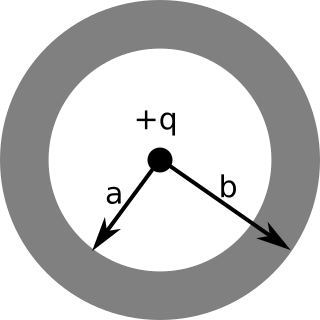
\includegraphics[width=0.3\linewidth]{./images/hw8/dielectric_shell.png}
\end{figure}

A point charge \(+Q\) is at the center of a spherical plastic shell
(inner radius \(a\), outer radius \(b\)) The shell is a \textbf{linear}
dielectric, with a dielectric constant \(\varepsilon_r\). The shell is
electrically neutral (it has no free charges).

\begin{enumerate}
\def\labelenumi{\arabic{enumi}.}
\tightlist
\item
  Compute \(\mathbf{E}\), \(\mathbf{D}\), and \(\mathbf{P}\)
  everywhere.\\
\item
  How is \(\mathbf{E}\) inside the plastic (\(a<r<b\)) different from
  what it would have been if the plastic were not present? (Explain
  why/how this difference arises physically.)
\item
  Sketch \(\mathbf{E}(r)\), briefly commenting on any interesting
  features.
\item
  Similarly, sketch \(\mathbf{D}(r)\).
\end{enumerate}

{\Large 4. Injecting free charges}\label{injecting-free-charges}

A solid sphere (radius \(R\)) of linear dielectric material (dielectric
constant \(\varepsilon_r\)) has been ``injected'' with a uniform free
charge density \(\rho_f\) throughout its volume.

\begin{enumerate}
\def\labelenumi{\arabic{enumi}.}
\tightlist
\item
  Find the potential at the center of the sphere (with \(V(\infty)=0\)).
  \emph{Hint: You might want to find D first.}
\item
  Does your answer come out larger or smaller than for a simple sphere
  of charge with uniform charge density \(\rho_f\) (that is, if you had
  neglected the effect of the dielectric constant)? Would that mean
  setting \(\varepsilon_r\) to 0, or to 1? Does this result make
  physical sense to you? Explain briefly.
\item
  What do you get in the limit of infinite dielectric constant? What
  physical situation does that limit remind you of?
\end{enumerate}

{\Large 5. Capacitor with
dielectric}\label{capacitor-with-dielectric}

You have a large (infinite in the \(x-y\) directions) parallel-plate
conductor (two big metal sheets, the upper one has free charge density
\(+\sigma\), the lower one \(-\sigma\)). The plates are a distance \(a\)
apart. The space between the sheets is half filled with a linear
dielectric oil with given dielectric constant \(\varepsilon_r = 4\).
Region I, (filling the top half of the volume) is vacuum. The lower
half, region II, is the dielectric oil. See the figure below.

\begin{figure}[htbp]
\centering
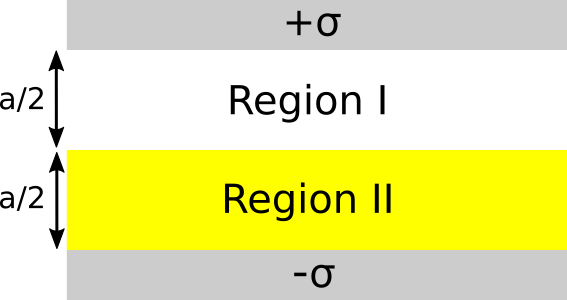
\includegraphics[width=0.4\linewidth]{./images/hw8/cap_w_dielectric.png}
\end{figure}

\begin{enumerate}
\def\labelenumi{\arabic{enumi}.}
\tightlist
\item
  Find \(\mathbf{D}\), \(\mathbf{E}\), and \(\mathbf{P}\) (direction and
  magnitude, giving all of them separately in regions I and II).
\item
  Find the location and amount of bound charge (surface and volume)
  everywhere.
\item
  Given this, go back and compute \(\mathbf{E}\) in region I and II to
  check your answers for part 1.
\item
  Find the voltage between the plates. If the plates are very large but
  not infinite, compare the capacitance before and after you added the
  dielectric oil. How does it compare with what you would get if you
  filled the entire region with that dielectric oil?
\end{enumerate}

{\Large 6. Magnetic Forces}\label{magnetic-forces}

\begin{enumerate}
\def\labelenumi{\arabic{enumi}.}
\tightlist
\item
  Griffiths works out (Ex 5.2) the general solution to motion of a
  particle in ``crossed E and B fields'' (\(\mathbf{E}\) points in the
  \(z\)-direction, \(\mathbf{B}\) in the \(x\)-direction) Work out his
  solution carefully, make sure you follow it. Then, use it to answer
  the following:
\item
  Suppose the particle starts at the origin at \(t=0\), with a given
  velocity \(\mathbf{v}(t=0) = v_0\hat{y}\). Use Griffiths' formal
  results (Eq. 5.6) to find the ``special initial speed'', \(v_0\),
  whose subsequent motion is simple straight-line constant-speed motion.
  Verify that this answer makes sense by using elementary Phys 184-style
  right-hand rule arguments and the Lorentz force law,
  \(\mathbf{F} = q (\mathbf{E} + \mathbf{v} \times \mathbf{B})\)
\item
  The discovery of the electron (J.J. Thomson, 1897) used an apparatus
  with crossed \(\mathbf{E}\) and \(\mathbf{B}\) just like the above.
  Thomson adjusted \(\mathbf{E}\) until he observed ``straight-line,
  constant-speed'' motion of the particle beam. Then, he turned off the
  \(E\)-field, and measured the radius of curvature (\(R\)) of the
  electron beam (deflected purely by the remaining \(B\)-field). Given
  \(E\), \(B\), and \(R\) (all measured), deduce Thomson's formula to
  find the charge to mass ratio (\(e/m\)) of the electrons.
\item
  Go back to Griffiths' Ex 5.2 again, but this time suppose your
  particle starts at the origin with \(\mathbf{v}(t=0) = v_1\hat{y}\),
  with starting speed \(v_1\) exactly \textbf{half} the ``special
  value'' velocity you found in part 2. Find and sketch the resulting
  trajectory of the particle. Is the kinetic energy of the particle
  constant with time? Briefly, comment (Is this consistent with energy
  conservation?!)
\end{enumerate}

{\Large 7. Current Densities}\label{current-densities}

We are going to be working with ``current densities'' for the rest of
the term. Let's start with a couple simple examples for you to practice
with.

\begin{enumerate}
\def\labelenumi{\arabic{enumi}.}
\tightlist
\item
  A solid cylindrical straight wire (radius \(a\)) has a current \(I\)
  flowing down it. If that current is uniformly distributed JUST over
  the outer surface of the wire (i.e.~none is flowing through the
  ``volume'' of the wire, it's all surface charge), what is the
  magnitude of the surface current density, \(\mathbf{K}\)?
\item
  Suppose that current does flow throughout the volume of the wire, but
  in such a way that the volume current density \(J\) grows
  quadratically with distance from the central axis. What is the formula
  for \(J\) everywhere in the wire? \emph{Note that neither situation i
  nor ii is physically what happens in normal wires!}
\item
  A DVD has been rubbed so that it has a fixed, constant, uniform
  surface electric charge density \(\sigma\) everywhere on its top
  surface. It is spinning at angular velocity \(\omega\) about its
  center (which is at the origin). What is the magnitude of surface
  current density \(\mathbf{K}\) at a distance \(r\) from the center?
\end{enumerate}
\end{document}
